% Elsevier version for Applied Energy (elsarticle, numbered references).
% The text lives in content/; the IEEE version is hp_sensitivity_overleaf.tex.
% Layout: [preprint,12pt] single column (submission). For a journal-like two-column proof use [5p,times,twocolumn].
%\documentclass[preprint,12pt]{elsarticle}
\documentclass[5p,times,twocolumn]{elsarticle}

\usepackage{amsmath}
\usepackage{amssymb}
\usepackage{graphicx}
\usepackage{adjustbox}
\usepackage{environ}% autotable (content/macros.tex)
\usepackage{tikz}
\usetikzlibrary{positioning,arrows.meta,calc}
\usepackage{textcomp}
\usepackage{booktabs}
\usepackage[hidelinks]{hyperref}
\usepackage{xurl}% long URLs in the references may break anywhere, so they stay inside the column
\urlstyle{same}% URLs and DOIs in the text font, not typewriter
\graphicspath{{figures/}}

% Figure width follows the layout chosen in \documentclass:
%   two-column (5p): one-column figures fit the column, as in the IEEE version;
%   one-column (preprint): figures at about the IEEE column width.
% Tables size themselves (autotable in content/macros.tex).
\newlength{\figw}
\makeatletter
\if@twocolumn
  \setlength{\figw}{\columnwidth}
\else
  \setlength{\figw}{0.6\textwidth}
\fi
\makeatother
% Shared macros for both templates (IEEE and Elsevier wrappers \input this file).
% Widths \figw (single-column figure) and \tabw (maximum table width) are set by each wrapper.
\definecolor{chgblue}{HTML}{0645AD}
\newcommand{\chg}[1]{#1}
% shared style of the two block diagrams (Figs. 1 and 5)
\tikzset{
  flow/.style={font=\footnotesize, >=latex},
  fin/.style={draw, fill=black!6, rounded corners=1pt, align=center, text width=22mm, minimum height=9mm, inner sep=2pt},
  fproc/.style={draw, rounded corners=3pt, align=center, text width=22mm, minimum height=9mm, inner sep=2pt},
  fout/.style={fproc, thick},
  flab/.style={font=\scriptsize, text=black!60, align=center},
}


% reference list in journal style: footnote size, tight spacing (natbib, loaded by elsarticle)
\renewcommand{\bibfont}{\footnotesize}
\setlength{\bibsep}{1pt plus 0.3ex}

% let tall floats sit near their text instead of drifting to the end
\renewcommand{\topfraction}{0.9}
\renewcommand{\bottomfraction}{0.8}
\renewcommand{\textfraction}{0.07}
\renewcommand{\floatpagefraction}{0.7}
\setcounter{topnumber}{3}
\setcounter{totalnumber}{5}

\journal{Applied Energy}

\begin{document}

\begin{frontmatter}

\title{Estimating the Installed Capacity of Aggregated Thermostatically Controlled Loads from Net Load and Temperature}

% TODO (authors): affiliations and the corresponding author's details
\author[aff1]{Alexandre M. V. Gouveia\corref{cor1}}
\ead{alexandremiguel.venanciogouveia@kuleuven.be}
\author[aff1]{Md. Umar Hashmi}
\author[aff1]{Reinhilde D'hulst}
\author[aff1]{Dirk Van Hertem}
\cortext[cor1]{Corresponding author}
\affiliation[aff1]{organization={TODO: department and organisation},
            city={TODO},
            country={Belgium}}

\begin{abstract}
The electrification of heating and cooling is connecting more thermostatically controlled loads (TCLs), such as heat pumps (HPs), to low-voltage networks. Distribution system operators (DSOs) need the installed TCL capacity behind each feeder to plan for cold-weather peaks, but rarely know it. This paper estimates this capacity from the feeder net load and outdoor temperature a DSO already holds, plus the temperature sensitivity of the simultaneity factor (SF). The SF is the share of installed capacity in use, and its sensitivity is how fast this share grows as the temperature falls. The SF sensitivity is calibrated once on a small pilot of households with submetered heating. Dividing the feeder's net-load sensitivity, the rate at which its net load grows as the temperature falls, by the SF sensitivity gives its installed capacity. On 1260 semi-synthetic aggregates of Swiss households, the capacity is recovered at a weighted absolute percentage error (WAPE) of 19\%, with the error growing as the share of households with an HP falls. On three real Swiss and German aggregates outside the pilot, where every household has an HP, the estimates lie within 10\% of the true capacity. The same data recover the temperature-driven HP energy, with no pilot, at a WAPE of 9\%, and a flexibility potential at a WAPE of 10\%. Across populations from five countries, the SF sensitivity transfers within 12\% inside one climate zone. It differs by 13--14\% between HP technologies, however, and up to 1.7-fold between climate zones and between social and private housing.

\end{abstract}

% Applied Energy: 3 to 5 highlights of at most 85 characters each, also submitted as a separate file (highlights.txt)
\begin{highlights}
% Applied Energy highlights: 3 to 5 bullets, at most 85 characters each (spaces included)
\item Installed heat-pump capacity is estimated from feeder net load and temperature
\item A simultaneity-factor sensitivity is calibrated once on a small submetered pilot
\item 9.5\% nMAE on 1260 semi-synthetic aggregates; within 10\% outside the pilot
\item The calibration transfers within one climate zone, not across housing tenures
\item The same fits quantify the flexibility potential at a 4.8\% nMAE

\end{highlights}

% Applied Energy: 1 to 7 keywords
\begin{keyword}
Thermostatically controlled loads \sep heat pumps \sep low-voltage networks \sep simultaneity factor \sep installed capacity \sep flexibility \sep distribution system observability
\end{keyword}

\end{frontmatter}

% =====================================================================
\section*{Nomenclature}
\newcommand{\nomentry}[2]{\item[#1] #2}
\begin{list}{}{\setlength{\labelwidth}{2.6cm}\setlength{\leftmargin}{2.8cm}\setlength{\labelsep}{0.2cm}%
  \setlength{\itemsep}{0pt}\setlength{\parsep}{0pt}\renewcommand{\makelabel}[1]{#1\hfil}}
\nomentry{DER}{Distributed energy resource.}
\nomentry{DSO}{Distribution system operator.}
\nomentry{EV}{Electric vehicle.}
\nomentry{HP}{Heat pump.}
\nomentry{LV}{Low voltage.}
\nomentry{NILM}{Non-intrusive load monitoring.}
\nomentry{OLS}{Ordinary least squares.}
\nomentry{PV}{Photovoltaics.}
\nomentry{SF}{Simultaneity factor.}
\nomentry{TCL}{Thermostatically controlled load.}
\nomentry{nMAE}{Normalised mean absolute error.}
\nomentry{$P_{\mathrm{net}}$}{Aggregated net load.}
\nomentry{$P_{\mathrm{TCL}}$}{Aggregated TCL load.}
\nomentry{$P_{\text{non-TCL}}$}{Aggregated non-TCL load.}
\nomentry{$P_{\mathrm{base}}$}{Temperature-independent base load.}
\nomentry{$\hat{P}_{\mathrm{TCL}}^{\,i}$}{Fitted TCL load of aggregate $i$.}
\nomentry{$s_h,\ s_c$}{Heating, cooling sensitivities of the net-load fit.}
\nomentry{$T_h,\ T_c$}{Heating, cooling threshold temperatures.}
\nomentry{$T_{\mathrm{d}}$}{Design temperature.}
\nomentry{$P_{\mathrm{TCL}}^{\max}$}{TCL installed capacity.}
\nomentry{$P_k^{\max}$}{TCL installed capacity active in regime $k$.}
\nomentry{$\mathrm{SF}_h,\ \mathrm{SF}_c$}{Heating, cooling simultaneity factor.}
\nomentry{$\hat{\mathrm{SF}}_h,\ \hat{\mathrm{SF}}_c$}{Fitted heating, cooling simultaneity factor.}
\nomentry{$b_h,\ b_c$}{SF intercepts at the threshold temperatures.}
\nomentry{$m_h,\ m_c$}{Heating, cooling SF sensitivities.}
\nomentry{$R^2_h,\ R^2_c$}{Coefficient of determination of a fit on the days of the heating, cooling regime.}
%\nomentry{$T_h^{\mathrm{SF}},\ T_c^{\mathrm{SF}}$}{Heating, cooling threshold temperatures of the SF fit.}
\nomentry{$\alpha_F$}{Flexibility duty cycle.}
\nomentry{$\Delta t$}{Energy integration period.}
\nomentry{$\Delta t_{Th}$}{Thermal-inertia window.}
\nomentry{$E_{\mathrm{TCL}}$}{Temperature-driven TCL energy.}
\nomentry{$E_{\mathrm{flex}}$}{Flexible energy.}
\nomentry{$N,\ N_{hp}$}{Number of households and heat pumps.}

\end{list}

% =====================================================================
\section{Introduction}
\label{sec:intro}

The electrification of residential heating and cooling is a central lever of decarbonisation policy. Its devices are thermostatically controlled loads (TCLs), such as heat pumps (HPs), electric resistance heaters and air conditioners, and the HP leads their uptake \cite{Iea22}. In 2025, about 2.9 million HPs were sold in 21 European countries, which brought the installed stock to 29.3 million \cite{Ehp26}. On 200 German low-voltage (LV) feeders, installed HP power rose by over 20\% from 2023 to 2025 \cite{Tre26}.

The demand of these devices follows the outdoor temperature, and their uptake loads LV networks that may not have been sized for this load. Field and simulation studies show that TCLs raise the coincident peak of feeders and transformers, i.e.\ the highest load their devices draw together, in extreme weather. HPs are the most studied case, with the sharpest peak in cold spells, when many devices run at once \cite{Vel11, Akm14, Som21, Bec24, Lia26}. Electric vehicles (EVs) add further load to the same feeders \cite{Bec24}.

A DSO needs the installed capacity of the TCLs behind each feeder, rather than only their coincident peak, for three reasons. First, the installed capacity scales with adoption, so it supports planning scenarios as the number of TCLs grows. Second, the installed capacity bounds the peak the TCLs can draw when they are synchronised. Third, network planning sizes transformers and cables for a design peak. This design peak is the installed capacity multiplied by the simultaneity factor (SF), the share of the installed capacity drawn at once \cite{Few24}. For HPs, it is set by cold weather, when their coincident demand peaks \cite{Lov17, Che21b, Rou23}. The SF also bounds the flexibility the TCLs can offer \cite{Mul19, Zir19, Dhu15}, since only the capacity not in use can be switched on.

A DSO rarely knows this capacity. Privacy concerns and limits on metering and data exchange restrict the DSO's access to household data, and its records of distributed energy resources (DERs) are often incomplete or out of date \cite{Gou26}. What the DSO does hold is the net load metered for a collection of households, such as those supplied by a substation. This paper calls such a metered point, together with the households behind it, an aggregate. Where smart meters are rolled out, the DSO also meters each household, but its access to these data is often restricted. The DSO usually knows how many households each feeder serves \cite{Tre26}. The installed capacity of the TCLs behind a feeder therefore stays largely unobserved.

\begin{table*}[t]
\centering
\caption{Prior work on detecting and quantifying DERs and TCLs}
\label{tab:litreview}
\footnotesize\setlength{\tabcolsep}{2.4pt}
\resizebox{\textwidth}{!}{%
\begin{tabular}{llllllcccc}
\toprule
 &  &  &  &  &  &  & \multicolumn{2}{c}{Submetering needed} &  \\
\cmidrule(lr){8-9}
Reference & DER & Task & Level & Method & Input & \begin{tabular}[b]{@{}c@{}}Installed\\capacity\end{tabular} & Target & Training & Transferable \\
\midrule
\multicolumn{10}{l}{\textit{Detection and disaggregation}} \\
\cite{Fei13} & HP & Detection & Meter & ML (PU learning) & Smart meter &  &  & \checkmark &  \\
\cite{Wei20b} & HP & Detection & Meter & ML & Smart meter + weather &  &  & \checkmark &  \\
\cite{Bru23} & HP & Disaggregation & Meter & ML (deep) & 15-min smart meter &  &  & \checkmark &  \\
\cite{Gis26} & HP & Detection + disaggregation & Meter & ML (CNN) & Smart meter &  &  & \checkmark &  \\
\cite{Jar22} & PV/EV & Detection + disaggregation & Meter & ML & Net demand &  &  & \checkmark &  \\
\cite{Wan20} & PV/EV & Regional NILM, PV capacity & Substation & Signal processing & Substation load + irradiance & \checkmark &  &  &  \\
\cite{Oma24} & EV/HP/PV & Disaggregation & Substation & ML (deep) & Substation load &  &  & \checkmark &  \\
\cite{Led18} & AC & Real-time disaggregation & Feeder & Online learning & Feeder load + device models &  &  & \checkmark &  \\
\midrule
\multicolumn{10}{l}{\textit{Temperature-response models}} \\
\cite{Ali11} & Cooling & Change-point model & Community & Change-point & Aggr.\ load + temp. &  &  &  &  \\
\cite{Per17b} & AC & Change-point model & Meter & Change-point & Submetered AC + temp. &  & \checkmark &  &  \\
\cite{Mac19} & Sector load & Weather effects & System & Regression & Sector load + weather &  &  &  &  \\
\midrule
\multicolumn{10}{l}{\textit{TCL aggregate modelling}} \\
\cite{Mat13} & TCL & State estimation, control & Population & Markov model + Kalman filter & Aggr.\ load + TCL model &  &  &  &  \\
\cite{Hao15} & TCL & Flexibility (virtual battery) & Population & Physics (thermal) & TCL parameters + temp. &  &  &  &  \\
\midrule
\multicolumn{10}{l}{\textit{PV capacity}} \\
\cite{Zha16b} & PV & Detection + capacity & Meter & Statistical & Smart meter + cloud cover & \checkmark &  &  &  \\
\cite{Li19d} & PV & Capacity + energy & Meter & ML & Smart meter & \checkmark &  & \checkmark &  \\
\cite{Sos17} & PV & Disaggregation & Feeder & Physics & Power flow + GHI &  &  &  &  \\
\cite{Was21} & PV & Capacity & Feeder & Probabilistic & Aggr.\ net load & \checkmark &  &  &  \\
\cite{gouveia2026pvcapacity} & PV & Capacity & Substation & ML / model-based & Aggr.\ net load + GHI & \checkmark &  & \checkmark & \checkmark \\
\midrule
\multicolumn{10}{l}{\textit{HP demand, coincidence and flexibility}} \\
\cite{Bec24} & PV/EV/HP & Coincidence / impact & Feeder & Empirical & Smart-meter profiles &  &  &  &  \\
\cite{Lov17} & HP & Coincidence / ADMD & Population & Field study & Submetered HP &  & \checkmark &  &  \\
\cite{Che21b} & HP & Peak in cold weather & Population & Field study & Submetered HP &  & \checkmark &  &  \\
\cite{And20} & HP & Demand vs temperature & Population & Probabilistic & Submetered HP + temp. &  &  & \checkmark & \checkmark \\
\cite{And20b} & HP & Load profiles & Feeder & Data-driven thermal relation & Submetered HP + temp. &  &  & \checkmark & \checkmark \\
\cite{Rou23} & HP & Aggregated peak forecast & Transformer & Clustered load duration curves & Rated power + temp.\ + submetered HP &  &  & \checkmark & \checkmark \\
\cite{Mul19} & HP & Flexibility / DR & Population & Field study & Submetered HP &  & \checkmark &  &  \\
\cite{Dhu15} & Appliances & Flexibility / DR & Population & Field study & Submetered appliances &  & \checkmark &  &  \\
\midrule
This work & HP / TCL & Capacity, energy, flexibility & Aggregate & Change-point + SF & Net load + temp.\ + pilot SF & \checkmark &  & \checkmark & \checkmark \\
\bottomrule
\end{tabular}}
\begin{flushleft}
	\par\smallskip{\footnotesize 
		%Installed capacity: recovers the installed capacity. Submetering needed: submetered device data or labels are needed on the target aggregate itself (Target), or only to train or calibrate the method on other data, such as a submetered pilot (Training). Transferable: a calibration transfers to un-submetered aggregates. Level: individual meter; summed meters of an aggregate; feeder, substation or transformer measurement; or a submetered population. 
		AC: air conditioning; ADMD: after-diversity maximum demand; CNN: convolutional neural network; DER: distributed energy resource; DR: demand response; EV: electric vehicle; GHI: global horizontal irradiance; ML: machine learning; NILM: non-intrusive load monitoring; PU: positive-unlabelled; PV: photovoltaics.}
\end{flushleft}

\end{table*}


Five lines of research address this unobserved capacity, summarised in Table~\ref{tab:litreview}. Non-intrusive load monitoring (NILM) and HP detection recover thermostatic load from customer meters, either as a present-absent label \cite{Fei13, Wei20b, Ray19} or as a disaggregated energy time series \cite{Bru23, Gis26}. Some of these methods extend to LV substations \cite{Wan20, Oma24}, validated mostly on synthetic rather than measured substation aggregates. They need labelled or submetered training data, however, and stop short of the installed capacity.

Change-point and degree-day models fit load as a piecewise-linear function of temperature, from building-level formulations \cite{Fel08, Ruc92, Kis04}, reviewed in \cite{Faz16}, to aggregated and smart-meter populations \cite{Ali11, Per17b, Mac19}. They recover heating and cooling sensitivities and a threshold temperature without any labels. They stop, however, at the coincident response and never reach the installed capacity, the sum of the individual peak demands.

A separate body of work models aggregated TCL populations for control. These models describe a population through the thermal parameters of its devices. Callaway \cite{Cal09} uses such a model to make a population follow a load signal, and Hao et al.\ \cite{Hao15} represent a population as a stochastic battery whose power and energy limits bound its flexibility. The state of such a population can be estimated from its aggregate power \cite{Mat13}, and the air-conditioning demand of a feeder can be disaggregated in real time from feeder measurements \cite{Led18}. These methods assume known device models, or learn them from building- and device-level data, and none estimates how much TCL capacity is installed behind the meter.

For photovoltaics (PV) and other DERs, by contrast, installed-capacity estimation is well developed. Methods infer the capacity from aggregated net load or smart-meter data \cite{Was21, Liu22, Gou25, gouveia2026pvcapacity}. Irradiance plays the role there that temperature could play for TCLs, yet the TCL counterpart is largely missing \cite{Gou26}.

Studies of HP demand measure the coincident peak, as an after-diversity maximum demand, or model the coincidence factor, on submetered populations of known size \cite{Lov17, Che21b, Rou23}. Closest to this paper, Anderson et al.\ \cite{And20} fit a probabilistic model of HP demand against temperature to submetered customer data, to assess LV networks under a given HP penetration. Such models run forward, from a known number of HPs to the demand they cause, and none recovers the installed capacity behind a feeder whose households are not submetered.

To the best of the authors' knowledge, no prior method estimates the installed capacity of an aggregated TCL population from feeder-level net load without submetering the households of the target feeder. Change-point models observe the right signal but stop at the coincident response, and simultaneity studies reach the installed capacity only on submetered populations.

This paper joins the change-point and simultaneity approaches. It estimates the installed capacity from the net load and temperature of a feeder, together with the SF sensitivity, i.e.\ how fast the SF grows as the temperature falls. The SF sensitivity is calibrated once on a small pilot. The pilot is a set of households whose heating is submetered, i.e.\ metered separately from the rest of their load, so that their installed heating capacity can be measured. On the feeder under study, called the target, the net load also grows as the temperature falls, at a rate the DSO reads from its own data. This rate, the net-load sensitivity, is larger the more TCL capacity is installed behind the feeder. Dividing the net-load sensitivity of the target by the SF sensitivity of the pilot therefore gives the installed capacity of the target. The households of the target are never submetered, so one pilot serves many feeders.

The contributions of this paper are threefold.
\begin{enumerate}
\item \emph{Installed Capacity Estimation:} A method to estimate the installed TCL capacity behind a feeder from its net load and temperature, calibrated once on a small submetered pilot. The households of the target feeder are never submetered. On 1260 semi-synthetic Swiss aggregates, the capacity is recovered at a normalised mean absolute error (nMAE) of 9.5\%, or 7.5\% when the total number of households is known.
\item \emph{SF Sensitivity Transfer:} An evaluation of how far the SF sensitivity of a pilot transfers across populations. It holds at a median ratio of 1.00 between aggregates of one population, and within 10\% between regions of one country, 12\% between countries and 14\% between HP technologies. It differs by 1.65-fold between housing tenures and 1.7-fold between heating zones.
\item \emph{Flexibility Potential Estimation:} A method to quantify the flexibility potential of an aggregated TCL population against temperature, from the net-load sensitivity and the SF sensitivity. On the semi-synthetic Swiss aggregates, it recovers the annual flexible energy at an nMAE of 4.8\%.
\end{enumerate}

The rest of the paper is structured as follows: Section~\ref{sec:problem} introduces the net-load and SF fits and the transfer of the SF sensitivity; Section~\ref{sec:estimation} derives the installed capacity and the flexibility potential from them; Section~\ref{sec:data} describes the data and the evaluation design. Section~\ref{sec:results} reports the results, and Section~\ref{sec:discussion} discusses the error sources and limitations. Lastly, Section~\ref{sec:conclusion} concludes the paper. Fig.~\ref{fig:pipeline} maps each step of the method to the section that defines it.

\begin{figure}[t]
\centering
\adjustbox{max width=\figw}{%
\begin{tikzpicture}[flow]
% columns at x = 0, 28, 64 mm; rows at y = 0, -15, -30 mm
\node[fin]   (sub)  at (0, 0)         {Submetered pilot TCL load};
\node[fin]   (temp) at (0, -15mm)     {Outdoor temperature};
\node[fin]   (net)  at (0, -30mm)     {Aggregated net load};
\node[fproc] (sf)   at (28mm, 0)      {SF fit\\[-1pt]{\scriptsize\color{black!60}Sec.~\ref*{sec:fits-sf}}};
\node[fproc] (bath) at (28mm, -30mm)  {Net-load fit\\[-1pt]{\scriptsize\color{black!60}Sec.~\ref*{sec:fits-net}}};
\node[fout]  (cap)  at (64mm, 0)      {Installed capacity\\[-1pt]{\scriptsize\color{black!60}Sec.~\ref*{sec:uc-capacity}}};
\node[fout]  (fl)   at (64mm, -15mm)  {Flexibility\\[-1pt]{\scriptsize\color{black!60}Sec.~\ref*{sec:uc-flex}}};
\node[fproc] (en)   at (64mm, -30mm)  {Baseline energy\\[-1pt]{\scriptsize\color{black!60}Sec.~\ref*{sec:uc-flex}}};
\draw[->] (sub) -- (sf);
\draw[->] (temp.east) -- (sf.south west);
\draw[->] (temp.east) -- (bath.north west);
\draw[->] (net) -- (bath);
\draw[->] (sf) -- (cap) node[midway, above, flab, text=black] {SF\\sensitivity};
\draw[->] (bath.north east) -- (cap.south west);
\draw[->] (bath) -- (en);
\draw[->] (cap) -- (fl);
\draw[->] (en) -- (fl);
\end{tikzpicture}%
}
\caption{Overview of the method, with the section that defines each step. Section~\ref{sec:results} evaluates the two outputs.}
\label{fig:pipeline}
\end{figure}

% =====================================================================
\section{Problem and Approach}
\label{sec:problem}
\label{sec:fits}

For the TCLs within an aggregate, this paper estimates two quantities: their installed capacity and their flexibility potential. Both need the net load of the aggregate and the outdoor temperature, held by the DSO, and the SF sensitivity, calibrated once on a submetered pilot (Section~\ref{sec:transfer}). The flexibility builds on the temperature-driven TCL energy, which the net-load fit gives without a pilot.

The net load is the sum of a TCL and a non-TCL component,
\begin{equation}
P_{\mathrm{net}}(t) = P_{\mathrm{TCL}}(t) + P_{\text{non-TCL}}(t),
\label{eq:decomp}
\end{equation}
where $t$ denotes time and only the TCL component responds directly to temperature. The non-TCL component also carries a weaker, indirect temperature dependence, visible in the whole-home energy signature \cite{Wes20}. Still, TCLs dominate the total temperature response, so the model neglects the non-TCL contribution. On average, each household adds small non-TCL sensitivities $s_{n,h}$ and $s_{n,c}$ [kW/$^\circ$C] to the heating and cooling arms, so the neglected term grows with the household count $N$ and weighs most where few households hold a TCL. Section~\ref{sec:uc-capacity} gives an optional correction, and Section~\ref{sec:res-capacity} sizes the effect.

Two fits describe how the TCLs of an aggregate respond to the outdoor temperature. The first, the net-load fit, uses only the net load and temperature the DSO holds (Section~\ref{sec:fits-net}). The second, the SF fit, needs the submetered TCL load and installed capacity, which in practice only a pilot provides (Section~\ref{sec:fits-sf}). Both fits share the same piecewise-linear form and use daily means.

\subsection{Net-Load Fit}
\label{sec:fits-net}

When an aggregate's net load is averaged over each day and plotted against the daily mean temperature, it follows a piecewise-linear pattern. The load is roughly flat on mild days, and rises close to linearly as the temperature falls below, or rises above, a threshold.
 The net-load fit expresses the aggregated net load of \eqref{eq:decomp} as
\begin{equation}
\hat{P}_{\mathrm{net}}(T) = P_{\mathrm{base}} + s_h \max(0, T_h - T) + s_c \max(0, T - T_c),
\label{eq:bathtub}
\end{equation}
where $T$ is the daily mean temperature [$^\circ$C], $P_{\mathrm{base}}$ the temperature-independent load [kW] and $s_h$ and $s_c$ the heating and cooling sensitivities [kW/$^\circ$C]. The heating and cooling threshold temperatures $T_h \le T_c$ [$^\circ$C], also known as balance-point temperatures, bound a dead band over which no thermal response is present. The parameters of the fitted curve are computed through Ordinary Least Squares (OLS), with $T_h$ and $T_c$ chosen as the values that minimise the squared residuals of the entire fit. The two temperature-dependent segments, called the heating and cooling arms of the fit, form the fitted aggregated TCL load.

Fig.~\ref{fig:austin}(a) shows the net-load fit to aggregated Austin smart-meter data \cite{pecanstreet}, with the parameters of \eqref{eq:bathtub} marked. The thresholds divide the temperature axis into three regimes: the heating regime below $T_h$, the cooling regime above $T_c$ and the dead band between them, where the population neither heats nor cools. This work characterises the heating and cooling regimes alike and leaves the dead band out of scope. The evaluation of Section~\ref{sec:results} covers the heating regime only, since the available data allow no test of the transfer in the cooling regime (Section~\ref{sec:discussion}).

\begin{figure}[t]
\centering
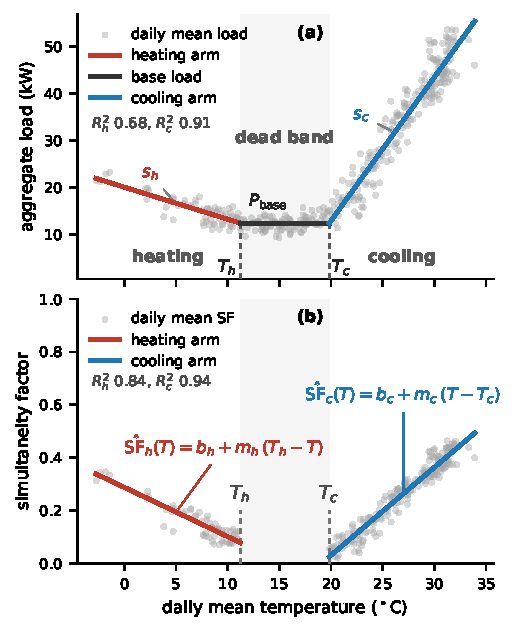
\includegraphics[width=\figw]{figures/fig_austin_fits.pdf}
\caption{The two fits of one aggregate of air-conditioned and furnace-heated households in Austin, Texas \cite{pecanstreet}. (a) Net-load fit \eqref{eq:bathtub} to the daily mean load, with the heating regime, dead band and cooling regime. (b) SF fit \eqref{eq:sffit} to the TCLs of the same households, with each daily point normalised by the installed capacity of the TCLs active in its regime \eqref{eq:sf-piecewise}. $R^2_h$ and $R^2_c$ score each arm on the days of its own regime.}
\label{fig:austin}
\end{figure}

From \eqref{eq:bathtub}, the temperature-driven component of the aggregated load of an aggregate $i$, with its own fitted parameters, is
\begin{equation}
\hat{P}_{\mathrm{TCL}}^{\,i}(T) = s_h^{\,i}\,\max(0, T_h^{\,i} - T) + s_c^{\,i}\,\max(0, T - T_c^{\,i}).
\label{eq:tclfit}
\end{equation}

The fitted parameters carry a physical interpretation. The threshold temperatures $T_h$ and $T_c$ mark where the population, on average, begins to heat or cool. They reflect both its buildings and its habits. Individual households start heating or cooling at different temperatures. Once many are aggregated, these differences average out, and $T_h$ and $T_c$ settle at values typical of the region (Section~\ref{sec:cross}).

The sensitivities $s_h$ and $s_c$ of the net-load fit measure how much heating or cooling load the population adds per degree.
They scale with the TCL capacity installed behind the meter, so an aggregate with more TCLs shows a steeper arm, all else being equal. Between aggregates of the same size, a steeper arm therefore also indicates a higher TCL penetration. Section~\ref{sec:res-capacity} confirms this, with $s_h$ tracking installed capacity across the aggregates.

The balance between $s_h$ and $s_c$ reflects the local climate. Hot regions are expected to be cooling-dominated, with $s_h \approx 0$, whereas regions with long winters, such as the Nordic countries, are heating-dominated, with $s_c \approx 0$.

\subsection{Simultaneity-Factor Fit}
\label{sec:fits-sf}

The SF is the ratio of the demand of a group of loads, here TCLs, at a given instant to the sum of their individual maximum demands. It reflects that connected devices do not all draw their full power at the same instant \cite{fani2024impact}. In distribution networks, the SF is central to planning. It lets DSOs size transformers, cables and protection for the peak the group actually draws, rather than for the sum of individual peaks.

Mathematically, the SF is the share of the aggregate's installed capacity drawn at a given temperature $T$,
\begin{equation}
\mathrm{SF}(T) = \frac{P_{\mathrm{TCL}}(T)}{P_{\mathrm{TCL}}^{\max}},
\label{eq:sf}
\end{equation}
where $P_{\mathrm{TCL}}(T)$ is the daily mean TCL load on a day of mean temperature $T$, and $P_{\mathrm{TCL}}^{\max}$ is the total installed capacity of the TCLs in the aggregate. Nameplate ratings are not available for most households, so the installed capacity of each TCL is taken as the peak of its submetered 15-min draw. The installed capacity of an aggregate is thus the summed peak draw of its TCLs, which tracks their rated power.

Since $P_{\mathrm{TCL}}(T)$ is a daily mean, the SF of this paper is a daily-mean SF. It is lower than the SF used in network planning, which takes the 15-min interval of highest aggregate demand; Section~\ref{sec:res-sf} gives the ratio between the two. The daily mean suits the aim of this paper, since the installed capacity follows from the SF sensitivity, and daily means reduce the effect of building thermal inertia \cite{Per17b}.

An aggregate may have a mix of TCLs with different behaviours with respect to temperature. Some TCLs, such as reversible HPs, can both heat and cool. Others only heat, such as resistive heaters, or only cool, such as air conditioners. Using the total TCL installed capacity in \eqref{eq:sf} would underestimate the SF, since cooling-only devices would still count towards the installed capacity in the heating regime, and \emph{vice versa}. Each regime therefore has its own capacity, defined as
\begin{equation}
    P_k^{\max} = \sum_{n\in \mathcal{N}_k}P_n^{\max},
\label{eq:pk}
\end{equation}
where $k$ denotes the regime (heating or cooling), $\mathcal{N}_k$ is the set of TCLs active in regime $k$, and $P_n^{\max}$ is the installed capacity of TCL $n$. The measured SF is then defined per regime as

\begin{equation}
\begin{aligned}
    \mathrm{SF}_h(T) &= {P_{\mathrm{TCL}}(T)}/{P_h^{\max}}, \quad \forall  T < T_h,\\
    \mathrm{SF}_c(T) &= {P_{\mathrm{TCL}}(T)}/{P_c^{\max}}, \quad \forall T > T_c,
\end{aligned}
\label{eq:sf-piecewise}
\end{equation}

with $h$ denoting heating and $c$ cooling. The SF is by definition bounded in $[0,1]$. The SF fit takes the same form as \eqref{eq:bathtub},
\begin{equation}
\begin{aligned}
    \hat{\mathrm{SF}}_h(T) &= b_h + m_h (T_h - T), \quad \forall T < T_h,\\
    \hat{\mathrm{SF}}_c(T) &= b_c + m_c ( T - T_c), \quad \forall T > T_c,
\end{aligned}
\label{eq:sffit}
\end{equation}
where $T_h$ and $T_c$ are the thresholds of the net-load fit \eqref{eq:bathtub} of the same aggregate. The SF fit does not fit thresholds of its own. It borrows them from the net-load fit, so both fits describe the same heating and cooling regimes. The intercepts $b_h$ and $b_c$ and the heating and cooling SF sensitivities $m_h$ and $m_c$ [1/$^\circ$C] are determined by OLS on the days of each regime. The intercepts capture the weather-independent share of TCL use, such as domestic hot water, which the net-load fit instead places in $P_{\mathrm{base}}$. The SF fit therefore needs the daily submetered TCL load, the installed TCL capacity per regime and the daily mean temperature, and in practice only a submetered pilot provides the first two (Section~\ref{sec:transfer}). Fig.~\ref{fig:austin}(b) shows the SF data points and the SF fit for the same Austin population.

The SF fit also links to the design peak of Section~\ref{sec:intro}. At a design temperature $T_{\mathrm{d}} < T_h$, the design SF is $b_h + m_h (T_h - T_{\mathrm{d}})$, and the installed capacity times this SF gives a daily-mean design load, which the 15-min design peak exceeds (Section~\ref{sec:res-sf}).

The observed SF stays well below 1. Each arm would reach the installed capacity of its regime, with every TCL drawing at once, only at temperatures well outside any observed weather. The gap between the observed TCL load and the installed capacity, the unused share $1-\mathrm{SF}$ of that capacity, is what the flexibility of Section~\ref{sec:flex} draws on.

\subsection{Cross-Dataset Characterisation}
\label{sec:cross}

\begin{autotable}[%
Climate: K{\"o}ppen--Geiger class~\cite{beck2018koppen}: Cfb, temperate oceanic; Dfa, Dfb, humid continental; Csb, warm-summer Mediterranean; Cfa, humid subtropical; BWh, hot desert. ASHP, GSHP, WSHP: air-, ground-, water-source HP; DHP: ductless (mini-split) HP; AC: air conditioning; ER: electric resistance heating.
\par\tnote{a}\,The SF uses the HPs' own draw only: Hennepin excludes the resistance backup, and WA and OR exclude the electric baseboard, furnace or other zonal heating circuits (17 of 22 and 16 of 21 households) that the net load includes.]
{Net-load and SF fits, one aggregate per dataset}{tab:cross}
\setlength{\tabcolsep}{3.5pt}
\begin{tabular}{llccccccccccccccccc}
\toprule
 & & & & \multicolumn{7}{c}{Net-load fit $\hat{P}_{\mathrm{net}}(T)$} & \multicolumn{8}{c}{SF fit $\hat{\mathrm{SF}}(T)$}\\
\cmidrule(lr){5-11}\cmidrule(lr){12-19}
dataset & TCL tech & $N$ & Climate & $P_{\mathrm{base}}$ & $s_h$ & $T_h$ & $R^2_h$ & $s_c$ & $T_c$ & $R^2_c$ & $b_h$ & $m_h$ & SF$^{\max}_h$ & $R^2_h$ & $b_c$ & $m_c$ & SF$^{\max}_c$ & $R^2_c$ \\
\midrule
Hamelin, DE~\cite{Sch22} & WSHP & 37 & Cfb & 16 & 3.9 & 13.9 & 0.72 & -- & -- & -- & 0.014 & 0.016 & 0.32 & 0.72 & -- & -- & -- & -- \\
Kloten, CH~\cite{Bru25,Kai26b} & ASHP, GSHP & 50 & Cfb & 54 & 6.1 & 16.5 & 0.92 & -- & -- & -- & 0.029 & 0.018 & 0.47 & 0.95 & -- & -- & -- & -- \\
%London, UK~\cite{lcl_heatpump} & ASHP & 9 & Cfb & 5 & 0.9 & 12.8 & 0.26 & -- & -- & -- & 0.123 & 0.022 & 0.34 & 0.26 & -- & -- & -- & -- \\
Oslo, NO~\cite{cofactor} & GSHP, ER & 849 & Dfb & 516 & 52.5 & 15.2 & 0.88 & -- & -- & -- & 0.106 & 0.022 & 0.70 & 0.80 & -- & -- & -- & -- \\
Hennepin, MN, US~\cite{resstock}\tnote{a} & ASHP & 150 & Dfa & 118 & 42.3 & 8.0 & 0.74 & -- & -- & -- & 0.061 & 0.022 & 0.46 & 0.93 & -- & -- & -- & -- \\
WA, US~\cite{neea_eulr}\tnote{a} & DHP, ER & 22 & Csb & 25 & 2.4 & 14.6 & 0.90 & 2.0 & 21.3 & 0.79 & 0.058 & 0.024 & 0.53 & 0.91 & 0.067 & 0.031 & 0.24 & 0.83 \\
OR, US~\cite{neea_eulr}\tnote{a} & DHP, ER & 21 & Csb & 25 & 2.1 & 13.3 & 0.87 & 2.0 & 21.8 & 0.75 & 0.044 & 0.023 & 0.46 & 0.91 & 0.097 & 0.024 & 0.22 & 0.79 \\
King, WA, US~\cite{resstock} & ASHP, ER & 150 & Csb & 146 & 21.1 & 13.3 & 0.89 & 11.0 & 18.4 & 0.93 & 0.036 & 0.036 & 0.53 & 0.90 & 0.091 & 0.038 & 0.37 & 0.96 \\
Austin, TX, US~\cite{pecanstreet} & AC, ER & 22 & Cfa & 12 & 0.7 & 11.2 & 0.68 & 3.0 & 19.8 & 0.91 & 0.078 & 0.019 & 0.34 & 0.84 & 0.025 & 0.033 & 0.49 & 0.94 \\
Maricopa, AZ, US~\cite{resstock} & ASHP, ER & 150 & BWh & 172 & 15.3 & 11.6 & 0.83 & 25.7 & 26.0 & 0.95 & 0.144 & 0.063 & 0.52 & 0.86 & 0.047 & 0.024 & 0.39 & 0.95 \\
\bottomrule
\end{tabular}
\end{autotable}

Both fits hold across climates. Table~\ref{tab:cross} reports them on aggregates from four countries, with each climate given as its K{\"o}ppen--Geiger class \cite{beck2018koppen}. The heating regime, the cooling regime or both are resolved as the local climate dictates (Fig.~\ref{fig:austin}(a)). Each fit is scored by its coefficient of determination on the days of its own regime, $R^2_h$ for heating and $R^2_c$ for cooling. In the heating regime, the net-load fit reaches an $R^2_h$ between 0.68 and 0.92 across the year-round aggregates. In the cooling regime, $R^2_c$ ranges from 0.95 in hot Maricopa to 0.75 in mild Oregon, where cooling is rare.

The threshold temperatures follow the local climate, whereas the net-load sensitivities follow the size of the aggregate. $T_h$ falls between 8 and 17\,$^\circ$C, and $T_c$ between 18 and 26\,$^\circ$C. A hot county such as Maricopa has a steep cooling arm, whereas a cold site such as Hamelin has no cooling. The sensitivities $s_h$ and $s_c$ of the net-load fit scale with the aggregate's total installed TCL capacity, and therefore with its size. The 849-household Norwegian aggregate and the electrified ResStock counties show the steepest arms for this reason. The SF sensitivities $m_h$ and $m_c$ remove this size dependence.

The SF sensitivities $m_h$ and $m_c$ group partly by K{\"o}ppen class \cite{beck2018koppen}. The two temperate oceanic (Cfb) aggregates, Hamelin and Kloten, sit at $m_h=0.016$ and $0.018\,^\circ$C$^{-1}$, and the two humid continental (Dfa and Dfb) sites, Oslo and Hennepin, near $0.022\,^\circ$C$^{-1}$, despite different HP technologies. The temperate dry and warm summer (Csb) class splits: its measured Washington and Oregon aggregates of ductless HPs sit at $0.023$--$0.024\,^\circ$C$^{-1}$, its simulated King County aggregate of ducted HPs with resistance backup at $0.036\,^\circ$C$^{-1}$. The cooling sensitivity $m_c$ spans $0.024$--$0.038\,^\circ$C$^{-1}$ without a clear grouping. The hot desert site, Maricopa, is the outlier, at $m_h=0.063\,^\circ$C$^{-1}$, possibly because few genuinely cold days anchor the coldest end of its heating arm. Across classes, $m_h$ varies by up to a factor of four, so the SF sensitivity is expected to transfer only within a climate class and TCL technology (Section~\ref{sec:transfer}). Section~\ref{sec:res-sf} tests this expectation on further populations with complete heating submetering.

\subsection{Transferability of SF}
\label{sec:transfer}

The method calibrates the SF sensitivity once on a submetered pilot and reuses it on every target. The SF fit needs submetered TCL data, which a DSO rarely holds for the aggregate under study. The pilot is a small set of households whose TCL load is submetered, so that its installed capacity is known. A target is an aggregate whose installed capacity is to be estimated and whose households are not submetered. In the main experiment, pilot and targets belong to the same population, i.e.\ the households of one dataset or study. In the experiments, a split is one random partition of a population into a pilot and targets.

Only the SF sensitivities $m_h$ and $m_c$ transfer. The pilot's thresholds follow its own building stock and climate, so the target's thresholds $T_h$ and $T_c$ are read from the target's net-load fit instead. The pilot's intercepts $b_h$ and $b_c$ describe weather-independent TCL use, which the target's net-load fit places in $P_{\mathrm{base}}$ and never attributes to its TCL arms.

The transfer rests on a hypothesis, which this paper tests rather than assumes: within a population, the SF sensitivity does not depend on the installed capacity or the TCL penetration of an aggregate. The hypothesis matters because the capacity estimate divides the target's net-load sensitivity by the pilot's SF sensitivity (Section~\ref{sec:uc-capacity}). Any mismatch between the pilot's and the target's SF sensitivity therefore passes directly into the estimated capacity. Section~\ref{sec:res-sf} tests it in three steps, each wider than the last: within one population, on aggregates outside the pilot and across populations from five countries.

\section{Aggregated TCL Quantification}
\label{sec:estimation}

The two fits, \eqref{eq:tclfit} and \eqref{eq:sffit}, are complementary. The net-load fit \eqref{eq:tclfit} needs no submetering, but its sensitivities also absorb any temperature response of the non-TCL load. The SF fit \eqref{eq:sffit} needs submetering but isolates the TCL simultaneity. Together they estimate two quantities a DSO needs about the TCLs of an aggregate: their installed capacity and flexibility potential. Installed capacity needs the transferred SF sensitivity, since the net load exposes the aggregated TCL demand, not the non-coincident sum of the individual peaks. Flexibility needs both fits: the net-load fit gives the temperature-driven energy the TCLs must deliver, and the SF fit the headroom above it. Section~\ref{sec:results} evaluates each quantity.

\subsection{Installed Capacity Estimation}
\label{sec:uc-capacity}

The installed capacity of each regime is the target's net-load sensitivity divided by the pilot's SF sensitivity, $s_k/m_k$. It is the sum of the individual peak demands \eqref{eq:pk}, which the aggregated TCLs never draw at once, so the net load never exposes it directly. The net-load fit does expose the temperature-driven TCL load $\hat{P}_{\mathrm{TCL}}^{\,i}(T)$ of aggregate $i$. Rearranging \eqref{eq:sf-piecewise}, the capacity of regime $k$ follows from this load and the SF at the same temperature.

The net-load arm and the SF must describe the same load. The net-load arm is zero at the aggregate's own threshold by construction, and the weather-independent TCL use sits in $P_{\mathrm{base}}$. The matching SF is therefore the temperature-driven part of \eqref{eq:sffit}. It starts from zero at the aggregate's own thresholds and grows with the pilot's SF sensitivity,
\begin{equation}
\begin{aligned}
    \hat{\mathrm{SF}}_h^{\,i}(T) &= m_h\,(T_h^{\,i} - T), \quad \forall T < T_h^{\,i},\\
    \hat{\mathrm{SF}}_c^{\,i}(T) &= m_c\,(T - T_c^{\,i}), \quad \forall T > T_c^{\,i}.
\end{aligned}
\label{eq:sf-target}
\end{equation}
Dividing the arms of \eqref{eq:tclfit} by \eqref{eq:sf-target} gives the installed capacity of each regime,
\begin{equation}
\begin{aligned}
    \hat{P}_h^{\max,i} &= \frac{s_h^{\,i}\,(T_h^{\,i} - T)}{m_h\,(T_h^{\,i} - T)} = \frac{s_h^{\,i}}{m_h}, \quad \forall T < T_h^{\,i},\\
    \hat{P}_c^{\max,i} &= \frac{s_c^{\,i}\,(T - T_c^{\,i})}{m_c\,(T - T_c^{\,i})} = \frac{s_c^{\,i}}{m_c}, \quad \forall T > T_c^{\,i}.
\end{aligned}
\label{eq:capacity}
\end{equation}
The temperature cancels, so the estimate needs no choice of evaluation day. The net-load fit supplies the numerator, which the DSO observes. The pilot supplies only the denominator $m_k$. The estimate is therefore as good as these two sensitivities, which Section~\ref{sec:results} tests.

The net-load sensitivities also hold the non-TCL response of the households, about $N s_{n,k}$ in regime $k$ (Section~\ref{sec:problem}), which biases \eqref{eq:capacity} upwards. A DSO that holds the net load of an aggregate without TCLs, for instance a feeder without HPs or air conditioners, can fit \eqref{eq:bathtub} to it at the target's thresholds and divide its sensitivities by its household count. This gives the non-TCL sensitivities per household, $s_{n,h}$ and $s_{n,c}$, which the corrected capacity of each regime subtracts,
\begin{equation}
\begin{aligned}
    \hat{P}_h^{\max,i} &= \frac{s_h^{\,i} - N^i s_{n,h}}{m_h}, & \hat{P}_c^{\max,i} &= \frac{s_c^{\,i} - N^i s_{n,c}}{m_c},
\end{aligned}
\label{eq:capacity-corr}
\end{equation}
where $N^i$ is the household count of aggregate $i$. On a target aggregate, the correction needs only its household count $N^i$, not which of its households hold a TCL.

% =====================================================================
\subsection{Flexibility Potential Estimation}
\label{sec:uc-flex}
\label{sec:flex}

The flexibility potential is the energy the TCL population can shift from its baseline consumption without breaching indoor thermal comfort \cite{Zir19}. Over a window $\Delta t_{Th}$, it equals $\hat{\mathrm{SF}}(T)\big(1-\hat{\mathrm{SF}}(T)\big)\,\hat{P}^{\max}\,\Delta t_{Th}$ \eqref{eq:flex-energy}. A DSO or an aggregator needs this energy for congestion management or to offer a flexibility product.

The baseline is the temperature-driven TCL energy, which follows from the net-load fit alone, with no pilot. Over a day of mean temperature $T$, it is given by
\begin{equation}
\hat{E}_{\mathrm{TCL}} = \left ( s_h \max(0, T_h - T) + s_c \max(0, T-T_c) \right ) \,\Delta t,
\label{eq:energy}
\end{equation}
with $\Delta t$ being the length of the period, here one day. Between $T_h$ and $T_c$ both arms are zero, so the baseline misses any TCL energy that persists into mild weather, such as domestic hot water.

How long a shift can last is set by the building stock, through a time window $\Delta t_{Th}$ within which the population must deliver a fixed thermal energy to stay comfortable. A larger $\Delta t_{Th}$ means a better-insulated building, or wider comfort bands \cite{Cha16}. Load-shifting studies of HPs treat this window the same way, as a property of the building \cite{Hon13}. In simulations of UK residential buildings, HP operation could be shifted by 1--2~h in the baseline case and by up to 6~h with much improved insulation and thermal buffering \cite{Hon13}. Building-stock insulation and indoor-comfort data are lacking, so $\Delta t_{Th}$ enters as an exogenous parameter of the building stock, held constant across temperatures, not as an output of the fits.

Over this window, the TCLs must still deliver the temperature-driven energy of \eqref{eq:energy}, drawn at the baseline power $\hat{P}_{\mathrm{TCL}}(T) = \hat{\mathrm{SF}}(T)\,\hat{P}^{\max}$,
\begin{equation}
\hat{E}_{\mathrm{TCL}}^{\Delta t_{Th}} = \hat{P}_{\mathrm{TCL}}(T)\,\Delta t_{Th} = \hat{\mathrm{SF}}(T)\,\hat{P}^{\max}\,\Delta t_{Th},
\label{eq:flex-baseline}
\end{equation}
where $\hat{\mathrm{SF}}$ and $\hat{P}^{\max}$ are those of the active regime, from \eqref{eq:sf-target} and \eqref{eq:capacity}. Their product equals the fitted TCL load of \eqref{eq:tclfit}, so the baseline is the temperature-driven load of the net-load fit. The schedule that delivers this same energy while deviating most from the baseline is the two-level square wave of Fig.~\ref{fig:flex-schedule}: full installed power $\hat{P}^{\max}$ for a fraction $\alpha_F$ of the window and zero for the rest. Its energy $\alpha_F\,\hat{P}^{\max}\,\Delta t_{Th}$ must equal \eqref{eq:flex-baseline}, which fixes the duty cycle at the simultaneity factor,
\begin{equation}
\alpha_F\,\hat{P}^{\max}\,\Delta t_{Th} = \hat{\mathrm{SF}}(T)\,\hat{P}^{\max}\,\Delta t_{Th} \;\Longrightarrow\; \alpha_F = \hat{\mathrm{SF}}(T).
\label{eq:flex-duty}
\end{equation}
The flexible energy is this schedule's symmetric deviation from the baseline. During the on phase the population draws $\hat{P}^{\max} - \hat{P}_{\mathrm{TCL}}$ above baseline for a time $\alpha_F \Delta t_{Th}$; during the off phase it curtails $\hat{P}_{\mathrm{TCL}}$ for a time $(1 - \alpha_F)\Delta t_{Th}$. The two areas are equal, giving an upward and downward flexible energy
\begin{equation}
E_{\mathrm{flex}} = \hat{\mathrm{SF}}(T)\big(1 - \hat{\mathrm{SF}}(T)\big)\,\hat{P}^{\max}\,\Delta t_{Th}.
\label{eq:flex-energy}
\end{equation}

The shiftable load comes from the net-load fit, and the transferred SF sets only the headroom above it, $1-\hat{\mathrm{SF}}(T)$. Since $\hat{\mathrm{SF}}(T)\,\hat{P}^{\max}$ equals the fitted TCL load, \eqref{eq:flex-energy} equals $\hat{P}_{\mathrm{TCL}}(T)\,\big(1-\hat{\mathrm{SF}}(T)\big)\,\Delta t_{Th}$, so the capacity estimate drops out. Since $E_{\mathrm{flex}}$ is linear in $\Delta t_{Th}$, Section~\ref{sec:res-flex} reports the normalised flexible energy $E_{\mathrm{flex}}/(P^{\max}\Delta t_{Th})$, with $P^{\max}$ the true installed capacity. Dividing by the window frees the results from a parameter that this paper takes as given rather than estimates. Dividing by the capacity makes aggregates with different numbers and sizes of HPs comparable.
\begin{figure}[t]
\centering
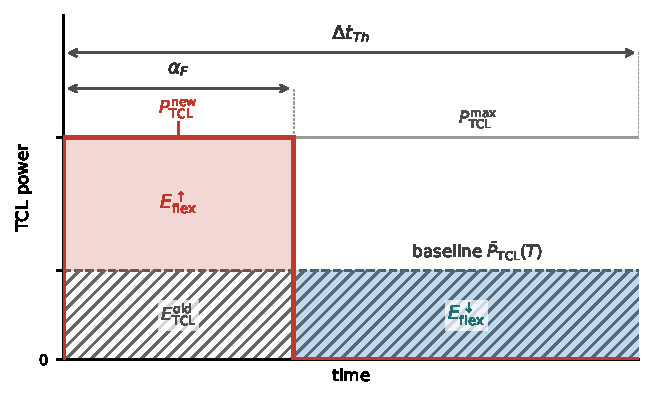
\includegraphics[width=\figw]{figures/fig_flex_schedule.pdf}
\vspace{-10pt}
\caption{The flexibility of \eqref{eq:flex-energy} over one cycle of the square-wave schedule. The aggregate must draw the baseline energy $E^{\mathrm{old}}_{\mathrm{TCL}} = \hat{P}_{\mathrm{TCL}}(T)\,\Delta t_{Th}$ (hatched) over the window. It can instead draw the same energy as the full-power pulse $P^{\mathrm{new}}_{\mathrm{TCL}}$ of duty cycle $\alpha_F = \hat{\mathrm{SF}}(T)$. The deviation from baseline is the flexible energy, equal upward ($E_{\mathrm{flex}}^{\uparrow}$) and downward ($E_{\mathrm{flex}}^{\downarrow}$).}
\label{fig:flex-schedule}
\end{figure}

This flexible energy is an idealised upper bound, not a dispatchable schedule. It takes the square wave as feasible and ignores each building's thermal state and the comfort limits within which its TCLs can shift. It therefore stands as a potential against temperature and window length, not as a firm reserve.

% =====================================================================
\section{Data and Evaluation Design}
\label{sec:data}

The evaluation draws on three sets of data, each further from the pilot. Semi-synthetic aggregates of one Swiss population test the full method against a known capacity (Section~\ref{sec:data-kloten}). Three aggregates outside the pilot test it on field meters (Section~\ref{sec:data-real}), and further populations with submetered heating test the SF transfer alone (Section~\ref{sec:data-pop}).

Two error metrics recur below. The nMAE scores the estimates $\hat{y}_i$ against their ground truth $y_i$ over a set $\mathcal{A}$ of $n$ aggregates,
\begin{equation}
	\mathrm{nMAE} =\sum_{i\in\mathcal{A}} \frac{ |\hat{y}_i - y_i|}{n\,\max_{j\in\mathcal{A}} y_j}100\%,
	\label{eq:nmae}
\end{equation}
i.e.\ the mean absolute error normalised by the largest true value in $\mathcal{A}$. A small aggregate, with a large percentage error but a small absolute error, therefore cannot dominate. Where a result is reported for a subset of the aggregates, $\mathcal{A}$ is that subset alone, so both the mean and the maximum are taken within it. The median ratio, the median of $\hat{y}_i / y_i$, gives the direction of the error, $< 1$ for an underestimate and $> 1$ for an overestimate. Every spread reported below is a 10--90\% range, i.e.\ it spans the 10th to the 90th percentile of the values across aggregates.

\subsection{Kloten Pilot and Semi-Synthetic Aggregates}
\label{sec:data-kloten}

The main experiment emulates a DSO that submeters one pilot and estimates the installed capacity of many feeders without submetering them. Each semi-synthetic aggregate plays the role of one such feeder. Its net load is known, and so is its true installed capacity, the sum of the capacities of its own HPs. The aggregates differ in size and HP penetration, so each has its own true capacity. For every aggregate, the estimate is its own net-load sensitivity divided by the pilot's SF sensitivity \eqref{eq:capacity}, scored against its true capacity.

The experiment draws on a single Swiss population, the households metered at the Kloten weather station in calendar 2023. The data combine two sources, the HEAPO dataset \cite{Bru25} and an additional smart-meter dataset \cite{Kai26b}. The load profiles have 15-min resolution, while the outdoor temperature is hourly. The only TCLs are HPs, and only heating is observed. The station holds 50 households with a submetered HP and 1307 households with neither an HP nor any other electric heating.

The 50 HPs are split at random into two halves of 25, 20 times over. In each split, the first half is the submetered pilot: its aggregated SF is fitted with \eqref{eq:sffit} and supplies the sensitivity $m_h$. Semi-synthetic aggregates, i.e. sums of measured households, are then drawn from the target half only, so no HP informs both the pilot and a target. Each aggregate combines $N_{hp}$ distinct HPs of that half, with the same households' other load, and $N - N_{hp}$ distinct households without an HP. The household count $N$ takes the values 10, 20, 30, 40 and 50, and $N_{hp}$ the values 5, 10, 15, 20 and 25, with $N_{hp} \le N$. Every feasible cell holds three aggregates per split, giving 1260 aggregates. All draws are without replacement, so no household recurs within an aggregate.

\subsection{Aggregates outside the Pilot}
\label{sec:data-real}

Three aggregates lie outside the Kloten pilot, each summed from its own field meters. Their submetered data serve only to validate the results, never as input. Two are regional aggregates: the HEAPO households of two further Swiss weather stations, Z{\"u}rich-Affoltern (Affoltern below) and Einsiedeln, with 21 and 6 submetered HPs. Their households share an area but not necessarily an LV network. The third comes from the WPuQ measurement campaign in Hamelin \cite{Sch22}. It is a real aggregate of 37 German single-family houses on one LV network, each with a submetered HP, and its net load is the sum of their individual meters. All three are summed rather than metered at a transformer, so they carry no network losses. They also contain no households without an HP, which makes their HP penetration 100\%. For these aggregates, the pilot comprises all 50 Kloten HPs.

\subsection{Populations with Submetered Heating}
\label{sec:data-pop}

The SF transfer is further tested on every population with submetered heating available to this study, beyond the one Swiss pilot. These are 849 Oslo apartments grouped in 10 blocks \cite{cofactor}, 182 households of the GB RHPP trial \cite{rhpp8151, Lov17} and US households of the BPA \cite{bpa_hphc} and NREL \cite{nrel_ccashp} field studies, whose submetering covers the HP and its backup heat. The BPA households lie in two heating zones, the milder western Washington (HZ1) and the colder inland (HZ2), where the NREL households also lie. The RHPP, BPA and NREL data hold the heating load of each household but no other load, so no faithful net load can be built from them. In Oslo, the apartments' own load includes electric heating that the submetered heating channel omits. Each row of Table~\ref{tab:transfer} therefore compares the target's own SF sensitivity with the pilot's, and the ratio minus one is the capacity error caused by the transfer alone.

% =====================================================================
\section{Results}
\label{sec:results}

\subsection{Installed Capacity}
\label{sec:res-capacity}

The net-load sensitivity grows with the installed capacity, as Section~\ref{sec:fits-net} anticipated. Fig.~\ref{fig:slope-capacity}(a) plots the fitted $s_h$ against the installed HP capacity across the aggregates, coloured by the number of HPs. The two track closely, at a Pearson correlation of 0.97, along a line through the origin of slope $0.020\,^\circ$C$^{-1}$. A steeper heating arm therefore signals more installed capacity.

\begin{figure}[t]
\centering
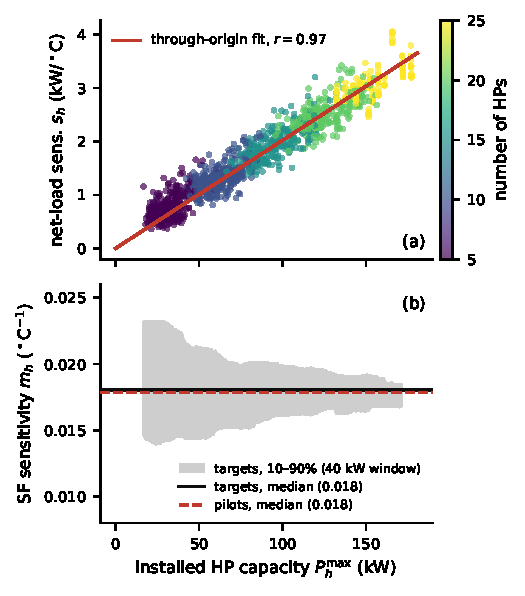
\includegraphics[width=\figw]{figures/fig_slope_capacity.pdf}
\caption{Sensitivities of the 1260 Kloten aggregates against installed HP capacity. (a) Fitted net-load sensitivity $s_h$, coloured by the number of HPs. (b) Own SF sensitivity $m_h$: 10--90\% range over a 40~kW rolling window, median of all aggregates and median of the 20 pilots.}
\label{fig:slope-capacity}
\end{figure}

With the pilot's SF sensitivity, \eqref{eq:capacity} recovers the installed capacity of the 1260 aggregates at an nMAE of 9.5\%, with a median overestimate of 16\%. In absolute terms, the mean error is 17~kW, the capacity of about three HPs of the mean 6.3~kW. The overestimate comes from the non-TCL temperature response that the net-load sensitivity absorbs, the neglected term of \eqref{eq:decomp}, sized below. The error shrinks as HPs are added: the nMAE falls from 22\% at five HPs to 13\% at 25, and the median overestimate from 35\% to 12\%.

\begin{figure}[t]
\centering
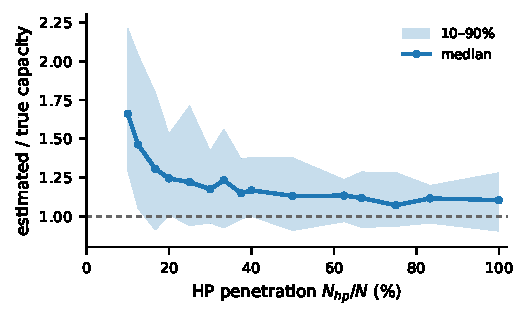
\includegraphics[width=\figw]{figures/fig_capacity_error.pdf}
\caption{Ratio of estimated to true installed capacity for the 1260 Kloten aggregates, against HP penetration $N_{hp}/N$, uncorrected \eqref{eq:capacity} and corrected with the known household count $N$ \eqref{eq:capacity-corr}: median and 10--90\% range at each penetration.}
\label{fig:capacity-error}
\end{figure}

Fig.~\ref{fig:capacity-error} shows the ratio of estimated to true capacity against the HP penetration. Its median falls from 1.66 at 10\% penetration to between 1.07 and 1.13 from 50\% on, and its 10--90\% range narrows from 1.30--2.21 to about 0.9--1.3 above 50\%. Below 15\% penetration, even the 10th percentile overestimates the capacity, by 5--30\%.

The overestimate grows as the penetration falls because $s_h$ also holds the non-TCL response of every household, about $N s_{n,h}$, while the TCL response grows only with $N_{hp}$. The pilot is not the cause: with each aggregate's own $m_h$, the median ratio still falls from 1.57 at 10\% penetration to 1.06 at 100\%.

The correction \eqref{eq:capacity-corr} removes most of this bias. Fitted on 50 households without an HP that no aggregate of the split contains, $s_{n,h}$ is a median 0.005~kW/$^\circ$C, against 0.112~kW/$^\circ$C for one HP. Subtracting this response cuts the median ratio at 10\% penetration from 1.66 to 1.19 and holds it within 1.00--1.11 from 15\% on. It lowers the nMAE from 9.5\% to 7.5\%. It leaves the spread, however, since a tenth of the households without an HP give 81\% of their response. The calibration households must hold no TCL: the steeper sensitivity of the pilot's other load, 0.011~kW/$^\circ$C, leaves the estimate a third too low at low penetration.

On all three aggregates outside the pilot, the capacity estimate lies within 10\% of the true capacity, at an nMAE of 3.8\%. It gives 112 against 109~kW at Affoltern ($+2\%$), 48 against 51~kW at Einsiedeln ($-6\%$) and 217 against 239~kW at Hamelin ($-9\%$). Einsiedeln holds only six HPs, below the 10 from which the Kloten aggregates give reliable estimates, so its result is indicative.

With each target's own SF sensitivity, the errors are $+6\%$, $+5\%$ and $+3\%$. The remaining error, which comes from the net-load sensitivity, stays small since every household in these aggregates has an HP.

\subsection{Transfer of the SF Sensitivity}
\label{sec:res-sf}

The capacity estimate divides the net-load sensitivity, which grows with the installed capacity, by the SF sensitivity, which should not. This subsection tests that the SF sensitivity does not grow with the capacity, the hypothesis of Section~\ref{sec:transfer}.

The SF fit is stable within the population. Because the SF comes from the submetered HPs alone, the households without an HP do not affect it. Fig.~\ref{fig:slope-capacity}(b) therefore plots the own $m_h$ of every aggregate against its installed capacity. It holds near $0.018\,^\circ$C$^{-1}$ at every capacity, at a Spearman correlation of $-0.06$, and the maximum heating SF holds near 0.47.
More HPs behind the meter do not shift these values but tighten them, as the 10--90\% range of $m_h$ narrows from 0.0092 at five HPs to 0.0023 at 25.

The daily-mean SF understates the 15-min SF of network planning. For the 50 Kloten HPs, the 15-min SF reaches 0.56 on the coldest day, 1.28 times the daily mean. This lies above the HP SF of 0.425 that a Great Britain-wide LV network study draws from UK field trials \cite{Few24}.

Across the 20 splits, the pilot's SF sensitivity $m_h$ has a median of $0.018\,^\circ$C$^{-1}$ and a 10--90\% range of 0.017--0.019. In one split, the pilot's SF fit at its own net-load threshold gives $\hat{\mathrm{SF}}_h(T) = 0.021 + 0.019\,(16.6 - T)$ for $T<16.6\,^\circ$C, at an $R^2_h$ of 0.94.

Placed at the target half's net-load threshold, the pilot's SF curve also reproduces the SF of the whole target half. Over 120 further random splits of the 50 HPs, it does so at a median $R^2_h$ of 0.91 and a 10--90\% range of 0.77--0.95. The pilot's SF sensitivity also recovers the capacity of the target half through \eqref{eq:capacity}. The median error is $+8\%$, with a 10--90\% range from $-8\%$ to $+27\%$.

Outside the pilot, the thresholds show why only the sensitivity transfers. The SF fit of the full Kloten pilot, at its own net-load threshold, is $\hat{\mathrm{SF}}_h(T) = 0.029 + 0.018\,(16.6 - T)$. The net-load thresholds of the targets are $16.7\,^\circ$C at Affoltern, $14.0\,^\circ$C at Einsiedeln and $13.9\,^\circ$C at Hamelin, against $16.6\,^\circ$C for the pilot. The threshold temperature varies with the insulation of the building stock, the internal gains from occupants and appliances and the preferred indoor setpoint \cite{Men18}. Transferring the full pilot curve from Kloten, intercept and threshold included, gives capacity errors of $-3\%$, $-20\%$ and $-26\%$. The error of the full curve therefore grows with the distance between the target's threshold and the pilot's, whereas the sensitivity alone stays within 10\%.

\begin{autotable}{Ratio of the target's own to the pilot's SF sensitivity [10--90\% range over random splits or a bootstrap over households]}{tab:transfer}
\setlength{\tabcolsep}{2.5pt}
\begin{tabular}{lccc}
\toprule
pilot $\rightarrow$ target & country & households & $m_h^{\mathrm{own}}/m_h^{\mathrm{pilot}}$ \\
\midrule
\multicolumn{4}{l}{\textit{Random splits}} \\
Kloten $\rightarrow$ Kloten & CH & 25/25 & 1.00 [0.85, 1.18] \\
Oslo $\rightarrow$ Oslo & NO & 5/5 blocks & 1.00 [0.84, 1.19] \\
RHPP $\rightarrow$ RHPP & GB & 10/10 & 1.00 [0.72, 1.39] \\
RHPP $\rightarrow$ RHPP & GB & 91/91 & 1.00 [0.89, 1.13] \\
BPA HZ1 $\rightarrow$ BPA HZ1 & US & 11/11 & 1.00 [0.80, 1.25] \\
BPA HZ2 $\rightarrow$ BPA HZ2 & US & 6/6 & 1.00 [0.69, 1.45] \\
\midrule
\multicolumn{4}{l}{\textit{Between studies, same country and climate zone}} \\
Kloten $\rightarrow$ Affoltern & CH & 50/21 & 0.97 [0.90, 1.06] \\
Kloten $\rightarrow$ Einsiedeln & CH & 50/6 & 0.90 [0.74, 0.99] \\
BPA HZ2 $\rightarrow$ NREL & US & 12/10 & 0.96 [0.85, 1.08] \\
NREL $\rightarrow$ BPA HZ2 & US & 10/12 & 1.05 [0.92, 1.19] \\
\midrule
\multicolumn{4}{l}{\textit{Between countries, same climate class (Cfb)}} \\
Kloten $\rightarrow$ Hamelin & CH$\rightarrow$DE & 50/37 & 0.88 [0.82, 0.94] \\
\midrule
\multicolumn{4}{l}{\textit{Between HP technologies}} \\
RHPP ASHP $\rightarrow$ RHPP GSHP & GB & 137/45 & 1.14 [1.08, 1.23] \\
RHPP GSHP $\rightarrow$ RHPP ASHP & GB & 45/137 & 0.87 [0.82, 0.94] \\
\midrule
\multicolumn{4}{l}{\textit{Between social and private housing}} \\
RHPP social $\rightarrow$ RHPP private & GB & 128/54 & 1.65 [1.58, 1.75] \\
RHPP private $\rightarrow$ RHPP social & GB & 54/128 & 0.61 [0.57, 0.64] \\
\midrule
\multicolumn{4}{l}{\textit{Between climate zones}} \\
BPA HZ1 $\rightarrow$ BPA HZ2 & US & 22/12 & 0.60 [0.54, 0.67] \\
BPA HZ2 $\rightarrow$ BPA HZ1 & US & 12/22 & 1.67 [1.51, 1.83] \\
\bottomrule
\end{tabular}
\end{autotable}

Table~\ref{tab:transfer} reports the transfer on the populations of Section~\ref{sec:data-pop}. Between random splits of one population, the ratio has a median of 1.00 in every dataset. Its spread narrows as the pilot and target grow, from a 10--90\% range of $-28\%$ to $+39\%$ at 10 RHPP households to $-11\%$ to $+13\%$ at 91. Between studies of one country and climate, the sensitivity transfers from the BPA HZ2 households to the NREL households within 5\%, and from Kloten to Affoltern and Einsiedeln within 10\%. From Kloten to Hamelin, across two countries of the same climate class, it transfers within 12\%.

The transfer degrades along three further axes. Between air- and ground-source HPs, the sensitivity differs by 13 to 14\%. Between the two BPA heating zones, it differs by a factor of 1.7. Between social and private housing within the RHPP trial, it differs by a factor of 1.65, far more than between the two technologies. This is possibly because the two housing tenures size their HPs differently against the heat demand of the building. That sizing sets how much of its capacity a population draws at a given temperature. A pilot therefore needs to match the target not only in climate and HP technology, but also in housing stock.

\subsection{Flexibility Potential}
\label{sec:res-flex}

The flexibility estimate recovers the annual flexible energy at an nMAE of 4.8\%, but its error changes sign with temperature. It overestimates the flexibility on the coldest days and underestimates it in mild weather, and both errors come mainly from the net-load fit, not from the transferred SF.

Across the 1260 aggregates, the ratio of estimated to actual annual flexible energy has a median of 1.04 and a 10--90\% range of 0.92--1.35. The estimate sums \eqref{eq:flex-energy} over the heating-regime days, each at its daily mean temperature, since the Kloten aggregates have no cooling regime. The actual covers the same days and applies the same expression to each hour's submetered SF and the true capacity, averaged over the day. The two share no input other than the HP load in the net load, so their agreement does not follow by construction.

The ratio splits into two factors, and the net-load fit sets most of it. The first, the energy factor, compares the baseline energy \eqref{eq:energy}, which the net-load fit gives with no pilot, with the submetered HP energy on the days below the threshold. It has a median ratio of 0.97, at an nMAE of 4.1\%. The second, the unused-capacity factor, has a median ratio of 1.07. About three percentage points of this factor come from the pilot's SF running slightly below the measured one. About four more come from the daily resolution of the estimate: computed from the daily mean SF, the actual would be 3\% higher and the median ratio 1.01, since $\mathrm{SF}(1-\mathrm{SF})$ is concave. The flexibility ratio and the energy factor correlate at 0.96. Since $\Delta t_{Th}$ cancels in the ratio, neither factor depends on the window.

\begin{figure}[t]
\centering
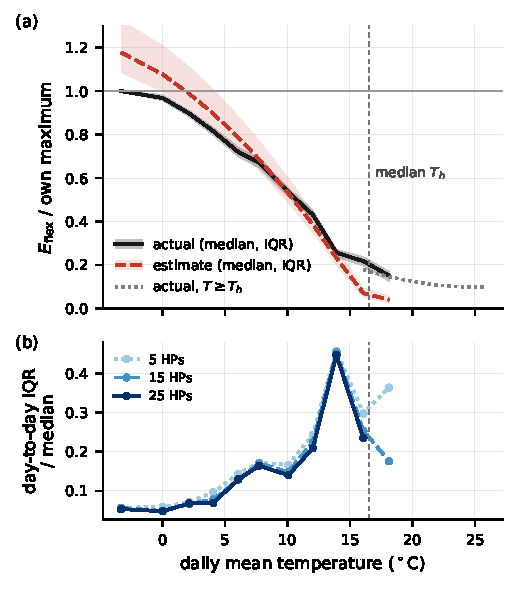
\includegraphics[width=\figw]{figures/fig_flex_normalised.pdf}
\caption{Normalised flexible energy $E_{\mathrm{flex}}/(P^{\max}\Delta t_{Th})$ against daily mean temperature, for the 1260 Kloten aggregates in 2~$^\circ$C bins, where $P^{\max}$ is the true installed capacity. Bottom: number of days of 2023 in each bin.}
\label{fig:flex-temperature}
\end{figure}

The annual ratio of 1.04 averages two opposite errors across temperature (Fig.~\ref{fig:flex-temperature}). The estimate overstates the flexible energy by 18\% on the coldest days and understates it by 9--11\% between 11 and 15~$^\circ$C. The estimate is closest to the actual, within 2\%, between 7 and 11~$^\circ$C, around the mean temperature of the heating days, 7.4~$^\circ$C.

On the coldest days, the fitted arm runs above the measured HP load. The measured load grows by about 0.02~kW per installed kW and degree down to 0~$^\circ$C, but by half that below it, whereas the fitted arm stays linear. The energy factor reaches 1.09 on these days, and the daily resolution and the pilot's SF add 4\% and 2\%. The capacity estimate plays no part, since it drops out of \eqref{eq:flex-energy}.

In mild weather, the estimate misses the HP use that does not depend on temperature, most plausibly hot-water heating \cite{Bru23}. The fitted arm reaches zero at $T_h$, whereas the measured HP load still draws 0.05--0.06~kW per kW installed at 14--16~$^\circ$C.

On the three aggregates outside the pilot, the flexibility ratio on the heating-regime days is 0.96 at Affoltern and 0.93 at Einsiedeln and Hamelin, slightly below the Kloten median of 1.04. It follows the energy factors of 0.89 to 0.92, while the unused-capacity factor stays between 1.01 and 1.05. These energy factors are lower than on Kloten possibly because these aggregates hold no households without an HP, whose temperature response inflates the heating arm.

% =====================================================================
\section{Discussion}
\label{sec:discussion}

\subsection{Error Sources and Transfer}
\label{sec:accuracy}

The capacity estimate carries two error sources. The first is the non-TCL temperature response that \eqref{eq:decomp} neglects, which biases the net-load sensitivity upwards and dominates at low HP penetration (Section~\ref{sec:res-capacity}). The second source is the pilot's SF sensitivity. Within Kloten, it matches the own SF sensitivity of each aggregate at a median ratio of 1.00, with a 10--90\% range of 0.84--1.22 across aggregates, so the transfer adds spread rather than bias. With each aggregate's own SF sensitivity, the nMAE is 7.1\%, against 9.5\% with the pilot's.

The sensitivity transfers within 12\% between populations that share a climate class and a housing stock (Table~\ref{tab:transfer}). The sensitivity differs by factors of 1.7 between heating zones and 1.65 between social and private housing, more than between HP technologies. Across the climate classes of Table~\ref{tab:cross}, it varies by up to a factor of four.

The pilot should therefore match the target in climate, HP technology and housing stock. A pilot of a few tens of HPs appears to suffice, since 25 Kloten HPs reproduce the SF of the other 25 (Section~\ref{sec:res-sf}). The pilot should, however, submeter every electric heating source of its households, including backup resistance heat. The target needs only the net load and outdoor temperature that the DSO already holds.

\subsection{Limitations}

Aggregates of the same Kloten split share HPs, so their errors are not independent, but the 20 splits keep the results from resting on any single partition. The three aggregates outside the pilot are few and all have an HP in every household, so lower HP penetrations are tested only on the semi-synthetic Kloten aggregates. This paper could not evaluate cooling, since the Washington pilot of the NEEA households \cite{neea_eulr}, the only aggregates with complete cooling ground truth, has no day above its cooling threshold in 2023.

The non-TCL temperature response, which the model neglects, is sized per household in Section~\ref{sec:res-capacity}. The resulting bias is thus predictable from the household count the DSO already holds, and Section~\ref{sec:uc-capacity} corrects it.

Deliberate HP control may also bias the estimate. Swiss and German domestic HPs commonly run under interruptible tariffs, under which the utility may cut their supply in blocking periods. Since 2024, {\S}14a of the Energy Industry Act (EnWG) also lets German DSOs throttle HPs above 4.2~kW \cite{Bna23}. Such control truncates the aggregated TCL peak and may bias the capacity estimate downwards. The aggregates outside the pilot may run under such tariffs, yet their estimates show no visible error from it.

% =====================================================================
\section{Conclusion}
\label{sec:conclusion}

This paper presents a method to estimate the installed capacity of the TCLs behind a feeder from its net load and outdoor temperature. The ratio of the net-load sensitivity of the feeder to the SF sensitivity gives the installed capacity, and only the SF sensitivity is calibrated, once, on a small submetered pilot. The capacity was recovered at an nMAE of 9.5\% on 1260 aggregates built from measured Swiss households, and within 10\% on two Swiss regional aggregates and a German LV network, where every household has an HP. Subtracting a per-household non-TCL sensitivity, fitted on households without TCLs, removes most of the overestimate and lowers the nMAE to 7.5\%. The estimates are least reliable on aggregates with a handful of HPs and most reliable once tens of HPs are aggregated, which is the regime a substation presents. The SF sensitivity transferred within one climate class but not between heating zones or between housing tenures, so the pilot should match the target in climate, HP technology and housing stock. The same fits give a flexibility potential at an nMAE of 4.8\%, overestimated by 18\% on the coldest days and underestimated in mild weather.

Four directions follow for future work. A wider and more diverse set of metered HPs, with every electric heating source submetered, would test the transfer on more populations and in the cooling regime. Data-driven methods for HP and TCL quantification should be evaluated against the proposed estimator, to see where a learned model earns its data cost. Recorded flexibility events would allow $\Delta t_{Th}$ to be calibrated against temperature and the TCLs' response to a call to be measured. Finally, modelling the TCL consumption that does not depend on temperature, chiefly domestic hot water, would close the gap between the estimated and the measured flexibility in mild weather.


% =====================================================================
% Declarations required by Applied Energy (TODO: authors to complete)
\section*{CRediT authorship contribution statement}
TODO.

\section*{Declaration of competing interest}
TODO.

\section*{Declaration of generative AI use}
TODO: required at submission (see the Applied Energy guide for authors).

\section*{Data availability}
TODO.

\section*{Acknowledgements}
TODO: funding sources and acknowledgements.

\bibliographystyle{elsarticle-num}
\bibliography{references}

\end{document}
